% !TeX spellcheck = en_EN
\documentclass[12pt, dvipsnames]{beamer}
\usepackage{appendixnumberbeamer}
\usepackage[T1]{fontenc}
\usepackage[utf8]{inputenc}
\usepackage{hyperref}
\usepackage{fontawesome5, lipsum}
\usepackage{graphicx}
\usepackage[english]{babel}
\usepackage{setspace, multicol, makecell, booktabs, multirow, relsize}
\usepackage{mtpro2, pifont}
\pdfmapfile{=mtpro2.map}
\usepackage{mathtools, amsthm, amsfonts, siunitx, physics, chemformula, empheq, bm}
\usepackage{appendixnumberbeamer}
\usepackage[backend=biber,
abbreviate=true,
doi=false,
isbn=false,
url=false,
eprint=false,
style=numeric-comp,
giveninits=true,
hyperref=true,
sorting=none,
date=year]{biblatex}
\usepackage{enumitem, csquotes, xurl}
\usepackage[most]{tcolorbox}
\usepackage{multimedia, tikz}
\usepackage[font=footnotesize, bf, format=plain, font=normalsize]{caption}
\usepackage[labelformat=simple]{subcaption}
\listfiles
\usepackage[absolute,overlay]{textpos}
\usepackage{tikz,circuitikz,pgfplots}

\graphicspath{ {./bilder/} }
\addbibresource{literatur.bib}

\AtEveryBibitem{\clearfield{pages}}

\renewcommand\thesubfigure{(\alph{subfigure})}
\usetikzlibrary{arrows.meta,positioning, calc, shapes, math, decorations.pathreplacing, decorations.markings, backgrounds,fit,matrix}
\usepgfplotslibrary{fillbetween}
\tcbuselibrary{breakable,skins}

\newcommand{\mycite}[1]{\tiny(\citefield{#1}{shortjournal}. \citeauthor{#1}. \citeyear{#1})}

\AtBeginDocument{\sisetup{per-mode = symbol, sticky-per, mode=text, text-font-command=\fontfamily{Times New Roman}\selectfont}}
\let\oldunit\unit
\renewcommand{\unit}[1]{\hspace{4pt}\oldunit{#1}}

% ------------------------------------------------------------------------------
% Use the beautiful metropolis beamer template
% ------------------------------------------------------------------------------
%\usepackage{FiraSans} 
\mode<presentation>
{
	\usetheme[progressbar=frametitle,background=light]{metropolis} 
	\usecolortheme{default} % or try albatross, beaver, crane, ...
	\usefonttheme[onlymath]{serif}  % or try serif, structurebold, ...
	\setbeamertemplate{navigation symbols}{}
	\setbeamertemplate{caption}[numbered]
	\setbeamertemplate{section in toc}[sections numbered]
	\setbeamerfont{frametitle}{size=\LARGE}
	\metroset{block=fill}
} 

\makeatletter
\setlength{\metropolis@progressinheadfoot@linewidth}{3pt}
\setlength{\metropolis@titleseparator@linewidth}{3pt}
\setlength{\metropolis@progressonsectionpage@linewidth}{3pt}

\makeatother

% ------------------------------------------------------------------------------
% tcolorbox / tcblisting
% ------------------------------------------------------------------------------	
% BEGIN_FOLD
\definecolor{MyBlue}{HTML}{0072B2}
\definecolor{MyOrange}{HTML}{D55E00}
\definecolor{MyRed}{HTML}{F00F0F}
\definecolor{MyGreen}{HTML}{2ca02c}
\definecolor{MyPurple}{HTML}{9467bd}
\definecolor{bgcolor}{HTML}{FAFAFA}
% END_FOLD

\def\npi{3.1415}
\pgfplotsset{
	compat=newest,
	MyStyle1/.style={
		width=\textwidth, height=4.5cm,
		set layers=axis lines on top,
		axis line style = {line width=1.3pt},
		xtick={-\npi,-\npi/2,...,5},
		ytick={-5,-4,...,5},
		xmin=-\npi, xmax=\npi,
		ymin=-0.2, ymax=4.8,
		xticklabels={$-\pi$,$-\frac{\pi}{2}$,\( 0 \), $\frac{\pi}{2}$,$\pi$},
		ymajorgrids=true,
		xmajorgrids=true,
		grid style={dashed, color=lightgray, line width=0.2pt},
		y label style={yshift=-1mm, xshift=-2mm	},
		x label style={yshift=1mm},
		tick style={draw=none},
	},
	every tick label/.append style={font=\scriptsize},
	every axis/.append style={font=\scriptsize},
	layers/axis lines on top/.define layer set={
		axis background,
		axis grid,
		axis ticks,
		axis tick labels,
		pre main,
		main,
		axis lines,
		axis descriptions,
		axis foreground,
	}{/pgfplots/layers/standard},
}

\makeatletter
\pgfcircdeclarebipolescaled{instruments}
{
	% put the node text above and centered
	\anchor{text}{\pgfextracty{\pgf@circ@res@up}{\northeast}
		\pgfpoint{-.5\wd\pgfnodeparttextbox}{
			\dimexpr.5\dp\pgfnodeparttextbox+.5\ht\pgfnodeparttextbox+\pgf@circ@res@up\relax
		}
	}
}
{\ctikzvalof{bipoles/oscope/height}}
{josephson}
{\ctikzvalof{bipoles/oscope/height}}
{\ctikzvalof{bipoles/oscope/width}}
{
	\pgf@circ@setlinewidth{bipoles}{\pgfstartlinewidth}
	\pgfextracty{\pgf@circ@res@up}{\northeast}
	\pgfextractx{\pgf@circ@res@right}{\northeast}
	\pgfextractx{\pgf@circ@res@left}{\southwest}
	\pgfextracty{\pgf@circ@res@down}{\southwest}
	\pgfmathsetlength{\pgf@circ@res@step}{0.25*\pgf@circ@res@up}
	\pgfscope
	\pgfpathrectanglecorners{\pgfpoint{\pgf@circ@res@left}{\pgf@circ@res@down}}{\pgfpoint{\pgf@circ@res@right}{\pgf@circ@res@up}}
	\pgf@circ@draworfill
	\endpgfscope
	\pgfscope
	\pgfpathmoveto{\pgfpoint{\pgf@circ@res@left}{\pgf@circ@res@up}}%
	\pgfpathlineto{\pgfpoint{\pgf@circ@res@right}{\pgf@circ@res@down}}%
	\pgfpathmoveto{\pgfpoint{\pgf@circ@res@right}{\pgf@circ@res@up}}%
	\pgfpathlineto{\pgfpoint{\pgf@circ@res@left}{\pgf@circ@res@down}}%
	\pgfusepath{draw}
	\endpgfscope
}
\def\pgf@circ@josephson@path#1{\pgf@circ@bipole@path{josephson}{#1}}
\tikzset{josephson/.style = {\circuitikzbasekey, /tikz/to path=\pgf@circ@josephson@path, l=#1},
		snake arrow/.style=
		{Latex-Latex,
			decorate,
			decoration={snake,amplitude=1mm,segment length=4mm,post length=3mm, pre length=5mm}}
}

\pgf@circ@declareground{myground}{0.6}{0.4}{
	\pgfsetlinewidth{\ctikzvalof{monopoles/ground/thickness}\pgfstartlinewidth}
	\pgfpathmoveto{\pgfpoint{-.6\pgf@circ@res@step}{0pt}}
	\pgfpathlineto{\pgfpoint{.6\pgf@circ@res@step}{0pt}}
	\pgfpathmoveto{\pgfpoint{-.4\pgf@circ@res@step}{-0.2\pgf@circ@res@step}}
	\pgfpathlineto{\pgfpoint{.4\pgf@circ@res@step}{-0.2\pgf@circ@res@step}}
	\pgfpathmoveto{\pgfpoint{-.25\pgf@circ@res@step}{-0.4\pgf@circ@res@step}}
	\pgfpathlineto{\pgfpoint{.25\pgf@circ@res@step}{-0.4\pgf@circ@res@step}}
	\pgfusepath{draw}
}
\makeatother

\newcommand*{\iu}{{i\mkern-1mu}}
\newcommand\supfrac[3][]{\mkern-2mu#1\frac{#2}{#3}\rule[-6pt]{0pt}{0pt}}

%BEGIN_FOLD
\ExplSyntaxOn
\NewDocumentCommand{\expo}{>{\SplitArgument{1}{/}} O{} >{\SplitArgument{1}{/}} O{} O{} }{%
	\ifthenelse{\equal{\use_i:nn#1}{-}}
	{\regex_match:nnTF {NoValue}{\use_ii:n#2}
		{\,\mathrm{e}^{\mkern-2mu\use_i:nn#1\rule[-6pt]{0pt}{0pt}\use_i:nn#2}}
		{\,\mathrm{e}^{\mkern-2mu\use_i:nn#1\frac{\use_i:nn#2}{\use_ii:nn#2}\rule[-6pt]{0pt}{0pt}#3}}
	}
	{\regex_match:nnTF {NoValue}{\use_ii:n#1}
		{\,\mathrm{e}^{\mkern-2mu\rule[-6pt]{0pt}{0pt}\use_i:nn#1}}
		{\,\mathrm{e}^{\mkern-2mu\frac{\use_i:nn#1}{\use_ii:nn#1}\rule[-6pt]{0pt}{0pt}\use_i:nn#2}}
}}

% uint function \uint[Interval]{function}{differential} (interval optional)
\NewDocumentCommand{\uint}{>{\SplitArgument{1}{,}}D[]{-,-} m m}{%
	\ifthenelse{\equal{\use_i:nn#1}{-}}
	{\int#2\, \dd#3}							% case 1: indefinite integral
	{\regex_match:nnTF {NoValue}{\use_ii:n#1}
		{\ifthenelse{\equal{\use_i:nn#1}{o}}
			{\oint #2\, \dd#3}					% case 2: Closed loop Integral
			{\int\c_math_subscript_token{\use_i:nn#1}#2 \dd#3}		% case 3: Volume/Surface Integral
		}
		{\int\limits\c_math_subscript_token{\use_i:nn#1}\c_math_superscript_token{\use_ii:nn#1}#2 \dd#3}	% case 4: Integral with boundaries
	}
}
\ExplSyntaxOff

\makeatletter
\newcommand*{\transpose}{%
	{\mathpalette\@transpose{}}%
}
\newcommand*{\@transpose}[2]{%
	% #1: math style
	% #2: unused
	\raisebox{\depth}{$\m@th#1\intercal$}%
}
\makeatother
%END_FOLD

\tikzset{fontscale/.style = {font=\relsize{#1}}}

\setstretch{1.5}
\usepackage{ragged2e}
\newtcolorbox{quotebox}{tikznode={align=left}, enhanced, colframe=MyOrange, top=0.2cm, bottom=0.2cm, colback=orange!15, right=0.1cm, left=0.1cm, hbox}
\newtcolorbox{mybox}[1]{enhanced, colframe=MyOrange, top=0.2cm, bottom=0.2cm, colback=bg, left=0.1cm, title=#1}

\title{Friday Talk\\[1em] \fullcite{dicarlo_demonstration_2009}}
\author{Alexander Helbok}
\date{\today}

\begin{document}
	\setstretch{1}
	\maketitle
	\setstretch{1.5}
%	##################### Intro #######################
	\begin{frame}{Overview}
		\begin{tikzpicture}[scale=2.25, every node/.style={scale=0.8, black}, every path/.style={line width=1.1pt}]
			\draw[line width=1.5pt] (-0.15, 0) -- (4.15, 0);
			
			\draw[MyBlue, fill](0,0) circle (.045) node [below, yshift=-0.2cm] {\Large\( 1990 \)};
			\draw[MyBlue, fill](1,0) circle (.045) node [below, yshift=-0.2cm] {\Large\( 1995 \)};
			\draw[MyBlue, fill](2,0) circle (.045) node [below, yshift=-0.2cm] {\Large\( 2000 \)};
			\draw[MyBlue, fill](3,0) circle (.045) node [below, yshift=-0.2cm] {\Large\( 2005 \)};
			\draw[MyBlue, fill](4,0) circle (.045) node [below, yshift=-0.2cm] {\Large\( 2010 \)};
			
			\draw[MyBlue] (0.8, 0) -- (0.8, 0.35) node [left, xshift=0cm] {Shor (1994)};
%			
			\draw[MyBlue] (1, 0) -- (1, 0.5) node [above left, xshift=0.5cm] {Trapped ion CNOT (1995)};
%			
			\draw[MyOrange] (1.8, 0) -- (1.8, 0.85) node [above left, xshift=0.5cm] {First SC qubit (1999)};
%			
			\draw[MyBlue] (2.8, 0) -- (2.8, 1.55) node [above left, xshift=0.5cm] {cQED (2004)};
%			
			\draw[MyBlue] (3.4, 0) -- (3.4, 1.9) node [above left, xshift=0.5cm] {Transmon (2007)};
%			
			\draw[MyPurple] (3.8, 0) -- (3.8, 2.4) node [above left, xshift=0.5cm] {2 qubit entanglement (2009)};
		\end{tikzpicture}
	\end{frame}
	
%	##################### Superconducting circuits #######################	
	\begin{frame}{Superconducting circuits}
		\begin{textblock*}{5cm}(.15\textwidth,.2\textheight)
			\begin{circuitikz}[scale=1, transform shape, every node/.style={font=\scriptsize}]
				\draw[line width=1.5pt, rounded corners=5pt] (1,0)
					to (2,0)
					to[american inductor, /tikz/circuitikz/bipoles/length=1cm, line width=0.8pt] (2, 2)
					to (1, 2)
					node[circ] {} to (0, 2)
					to[C, /tikz/circuitikz/bipoles/length=1cm] (0, 0)
					to (1, 0);
				\draw[line width=1.5pt] (1,0) -- (1,-0.2) node[myground, line width=0.8pt, /tikz/circuitikz/bipoles/length=1.8cm]{};

				\node[above] at (1, 2) {\( \phi \)};
				\node[right] at (0.3, 1) {\( C_r \)};
				\node[left] at (1.8, 1) {\( L_r \)};
			\end{circuitikz}
		\end{textblock*}
		
		\only<2->{
		\begin{textblock*}{5cm}(.5\textwidth,.2\textheight)
			\begin{circuitikz}[scale=1, transform shape, every node/.style={font=\scriptsize}]				
				\draw[line width=1.5pt, rounded corners=5pt] (1,0)
				to (2,0)
				to[color=MyBlue, josephson, /tikz/circuitikz/bipoles/length=0.8cm, line width=0.8pt] (2, 2)
				to (1, 2)
				node[circ] {} to (0, 2)
				to[C, /tikz/circuitikz/bipoles/length=1cm] (0, 0)
				to (1, 0);
				\draw[line width=1.5pt] (1,0) -- (1,-0.2) node[myground, line width=0.8pt, /tikz/circuitikz/bipoles/length=1.8cm]{};
				
				\node[above] at (1, 2) {\( \phi \)};
				\node[right] at (0.3, 1) {\( C_s \)};
				\node[above left] at (1.7, 1) {\( C_J \)};
				\node[below left] at (1.7, 1) {\( L_J \)};
			\end{circuitikz}
		\end{textblock*}}
		
		\only<3->{
		\begin{textblock*}{5cm}(.85\textwidth,.2\textheight)
			\begin{circuitikz}[scale=1, transform shape, every node/.style={font=\scriptsize}]				
				\draw[line width=1.5pt, rounded corners=5pt] (2,1.5)
				to (2,2)
				to (1, 2)
				node[circ] {} to (0, 2)
				to[C, /tikz/circuitikz/bipoles/length=1cm, line width=0.8pt] (0, 0)
				to (2, 0)
				to (2, 0.5);
				
				\draw[line width=1.5pt, rounded corners=3pt] (2, 0.5)
				to (2.5, 0.5)
				to[color=MyOrange, josephson, /tikz/circuitikz/bipoles/length=0.8cm, line width=0.8pt] (2.5, 1.5)
				to (1.5, 1.5)
				to[color=MyOrange, josephson, /tikz/circuitikz/bipoles/length=0.8cm, line width=0.8pt] (1.5, 0.5)
				to (2, 0.5);
				
				\draw[line width=1.5pt] (1,0) -- (1,-0.2) node[myground, line width=0.8pt, /tikz/circuitikz/bipoles/length=1.8cm]{};
				
				\node[above] at (1, 2) {\( \phi \)};
				\node[right] at (0.3, 1) {\( C_s \)};
%				\node[above right] at (2.3, 1) {\( C_J \)};
%				\node[below right] at (2.3, 1) {\( L_J \)};

	  			\draw[fill] (2, 1) circle (0.05);
	  			\draw[line width=1.2pt] (2, 1) circle (0.12) node [below, yshift=-0.05cm, xshift=0.1cm] {\scriptsize\( \Phi_\mathrm{ext} \)};
			\end{circuitikz}
		\end{textblock*}}
		
		\begin{textblock*}{5cm}(.07\textwidth,.6\textheight)
			\begin{tikzpicture}
				\begin{axis}[MyStyle1,
					scale=0.775,
					xlabel = phase \(\phi\),
					ylabel = {Energy (\oldunit{GHz})}]
					%Below the red parabola is defined
					\addplot[
					domain=-5:5,
					line width=1pt,
					samples=100,
					color=red,]
					{x^2};
					
					\foreach \i in {0.5, 1.5, 2.5, 3.5, 4.5}{
						\addplot [
						domain=-\i^0.5:\i^0.5,
						line width=1pt,
						samples=100,
						color=red,]
						{\i};}
					
					\addplot[domain=-0.5^0.5:0.5^0.5, red] {0.5} node[right,pos=1, black, xshift=1mm] {\( \ket{0} \)};
					\addplot[domain=-1.5^0.5:1.5^0.5, red] {1.5} node[right,pos=1, black, xshift=1mm] {\( \ket{1} \)};
					\addplot[domain=-2.5^0.5:2.5^0.5, red] {2.5} node[right,pos=1, black, xshift=1mm] {\( \ket{2} \)};
					
					\draw[{Stealth[width=2mm, length=1.7mm]}-{Stealth[width=2mm, length=1.7mm]}, line width=1.7pt, dash pattern=on 4pt off .85pt] (axis cs:0, 0.52) -- (axis cs:0, 1.48);
					\draw[{Stealth[width=2mm, length=1.7mm]}-{Stealth[width=2mm, length=1.7mm]}, line width=1.7pt, dash pattern=on 4pt off .85pt] (axis cs:0, 1.52) -- (axis cs:0, 2.48);
					\draw[{Stealth[width=2mm, length=1.7mm]}-{Stealth[width=2mm, length=1.7mm]}, line width=1.7pt, dash pattern=on 4pt off .85pt] (axis cs:0, 2.52) -- (axis cs:0, 3.48);
					%			\draw[{Stealth[width=2mm, length=1.7mm]}-{Stealth[width=2mm, length=1.7mm]}, line width=1.7pt, dash pattern=on 4pt off .85pt] (axis cs:0, 3.52) -- (axis cs:0, 4.48);
					
					\node[red] at (axis cs: 0,4) {QHO};
					
					\node[] at (axis cs: -2.2,2) {\( \hbar\omega_r \)};
				\end{axis}
			\end{tikzpicture}
		\end{textblock*}
		
		\only<2->{
		\begin{textblock*}{5cm}(.465\textwidth,.6\textheight)
			\begin{tikzpicture}
				\begin{axis}[MyStyle1,
					scale=0.775,
					xlabel = phase \(\phi\)]
					\addplot [
					dash pattern=on 10pt off 4pt,
					opacity=0.5,
					domain=-5:5,
					line width=1pt,
					samples=100,
					color=red,]
					{x^2};
					%						
					\addplot [
					domain=-5:5,
					line width=1pt,
					samples=100,
					color=MyBlue,]
					{-2.25*cos(deg(x))+2.25};
					%						
					\addplot[domain=-acos(1 - 0.5/2.25)*pi/180:acos(1 - 0.5/2.25)*pi/180,
					MyBlue, line width=1pt, opacity=1]
					{0.5} node[right,pos=1, black, xshift=1mm] {\( \ket{\mathbf{0}} \)};
					\addplot[domain=-acos(1 - (0.5+0.935)/2.25)*pi/180:acos(1 - (0.5+0.935)/2.25)*pi/180,
					MyBlue, line width=1pt, opacity=0.85]
					{0.5+0.935} node[right,pos=1, black, xshift=1mm] {\( \ket{\mathbf{1}} \)};
					\addplot[domain=-acos(1 - (0.5+0.935+0.864)/2.25)*pi/180:acos(1 - (0.5+0.935+0.864)/2.25)*pi/180,
					MyBlue, line width=1pt, opacity=0.7]
					{0.5+0.935+0.864} node[right,pos=1, black, xshift=1mm] {\( \ket{2} \)};
					\addplot[domain=-acos(1 - (0.5+0.935+0.864+0.78)/2.25)*pi/180:acos(1 - (0.5+0.935+0.864+0.78)/2.25)*pi/180,
					MyBlue, line width=1pt, opacity=0.55]
					{0.5+0.935+0.864+0.78} node[right,pos=1, black, xshift=1mm] {};
					\addplot[domain=-acos(1 - (0.5+0.935+0.864+0.78+0.62)/2.25)*pi/180:acos(1 - (0.5+0.935+0.864+0.78+0.62)/2.25)*pi/180,
					MyBlue, line width=1pt, opacity=0.4]
					{0.5+0.935+0.864+0.78+0.62} node[right,pos=1, black, xshift=1mm] {};
					
					\draw[MyBlue, {Stealth[width=2mm, length=1.7mm]}-{Stealth[width=2mm, length=1.7mm]}, line width=1.7pt, dash pattern=on 4pt off .85pt] (axis cs:0, 0.52) -- (axis cs:0, 0.5+0.915);
					\draw[MyBlue, {Stealth[width=2mm, length=1.7mm]}-{Stealth[width=2mm, length=1.7mm]}, line width=1.7pt, dash pattern=on 4pt off .85pt] (axis cs:0, 0.5+0.955) -- (axis cs:0, 0.5+0.935+0.844);
					
					\node[MyBlue] at (axis cs: 0,4.3) {Transmon};
					
					\node[] at (axis cs: -2.25,1.8) {\( \hbar\omega_{12} \)};
					\node[] at (axis cs: -2,0.9) {\( \hbar\omega_{01} \)};
				\end{axis}
			\end{tikzpicture}
		\end{textblock*}}
	
		\only<3>{
			\begin{textblock*}{5cm}(.77\textwidth,.6\textheight)
				\begin{tikzpicture}
					\begin{axis}[MyStyle1,
						scale=0.775,
						ylabel = \phantom{\( \delta \)Energy (\oldunit{GHz})},
						xlabel = phase \(\phi\)]
						\addplot [
						dash pattern=on 10pt off 4pt,
						opacity=0.5,
						domain=-5:5,
						line width=1pt,
						samples=100,
						color=red,]
						{x^2};
						%						
						\addplot [
						domain=-5:5,
						line width=1pt,
						samples=100,
						color=MyBlue,]
						{-2.25*cos(deg(x))+2.25};
						%						
						\addplot[domain=-acos(1 - 0.5/2.25)*pi/180:acos(1 - 0.5/2.25)*pi/180,
						MyBlue, line width=1pt, opacity=1]
						{0.5} node[right,pos=1, black, xshift=1mm] {\( \ket{\mathbf{0}} \)};
						\addplot[domain=-acos(1 - (0.5+0.935)/2.25)*pi/180:acos(1 - (0.5+0.935)/2.25)*pi/180,
						MyBlue, line width=1pt, opacity=0.85]
						{0.5+0.935} node[right,pos=1, black, xshift=1mm] {\( \ket{\mathbf{1}} \)};
						\addplot[domain=-acos(1 - (0.5+0.935+0.864)/2.25)*pi/180:acos(1 - (0.5+0.935+0.864)/2.25)*pi/180,
						MyBlue, line width=1pt, opacity=0.7]
						{0.5+0.935+0.864} node[right,pos=1, black, xshift=1mm] {\( \ket{2} \)};
						\addplot[domain=-acos(1 - (0.5+0.935+0.864+0.78)/2.25)*pi/180:acos(1 - (0.5+0.935+0.864+0.78)/2.25)*pi/180,
						MyBlue, line width=1pt, opacity=0.55]
						{0.5+0.935+0.864+0.78} node[right,pos=1, black, xshift=1mm] {};
						\addplot[domain=-acos(1 - (0.5+0.935+0.864+0.78+0.62)/2.25)*pi/180:acos(1 - (0.5+0.935+0.864+0.78+0.62)/2.25)*pi/180,
						MyBlue, line width=1pt, opacity=0.4]
						{0.5+0.935+0.864+0.78+0.62} node[right,pos=1, black, xshift=1mm] {};
						
						\draw[MyBlue, {Stealth[width=2mm, length=1.7mm]}-{Stealth[width=2mm, length=1.7mm]}, line width=1.7pt, dash pattern=on 4pt off .85pt] (axis cs:0, 0.52) -- (axis cs:0, 0.5+0.915);
						\draw[MyBlue, {Stealth[width=2mm, length=1.7mm]}-{Stealth[width=2mm, length=1.7mm]}, line width=1.7pt, dash pattern=on 4pt off .85pt] (axis cs:0, 0.5+0.955) -- (axis cs:0, 0.5+0.935+0.844);
						
						\node[MyBlue] at (axis cs: 0,4.3) {Transmon};
						
						\node[] at (axis cs: -2.25,1.8) {\( \hbar\omega_{12} \)};
						\node[] at (axis cs: -2,0.9) {\( \hbar\omega_{01} \)};
					\end{axis}
				\end{tikzpicture}
		\end{textblock*}}
		
		\only<4>{
		\begin{textblock*}{5cm}(.77\textwidth,.6\textheight)
			\begin{tikzpicture}
				\begin{axis}[
					scale=0.775,
					width=\textwidth, height=4.5cm,
					set layers=axis lines on top,
					axis line style = {line width=1.3pt},
					xlabel = flux bias \(\Phi_\mathrm{ext}\),
					ylabel = \( \delta \)Energy (\oldunit{GHz}),
					xtick={-1,-0.5,...,1},
					ytick={0,1,2,3,4,5},
					xmin=-1, xmax=1,
					ymin=-0.2, ymax=4.8,
					xticklabels={$-\pi$,$-\frac{\pi}{2}$, \( 0 \), $\frac{\pi}{2}$, \( \pi \)},
					ymajorgrids=true,
					xmajorgrids=true,
					grid style={dashed, color=lightgray, line width=0.2pt},
					y label style={yshift=-1mm, xshift=-2mm	},
					x label style={yshift=1mm},
					tick style={draw=none}]
					
					\node[MyOrange] at (axis cs: 0,4.3) {Split Transmon};
					
					\addplot[line width=0.8pt, orange, smooth] table [x=x, y=w01, col sep=comma] {bilder/asym_transmon_e.csv};
					\addplot[densely dotted, line width=0.8pt, MyRed, smooth] table [x=x, y=w02, col sep=comma] {bilder/asym_transmon_e.csv};
				\end{axis}
				
				\draw[line width=0.8pt, orange] (0.85, 0.6) --++ (0.3, 0) node [right] {\scriptsize \( \omega_{01} \)};
				\draw[densely dotted, line width=0.8pt, MyRed] (0.85, 0.25) --++ (0.3, 0) node [right] {\scriptsize \( \omega_{12} \)};
			\end{tikzpicture}
		\end{textblock*}}
	\end{frame}
	
	\begin{frame}{Die shot}
		\centering
		\begin{tikzpicture}
			\node[anchor=south west,inner sep=0] (image) at (0,0) {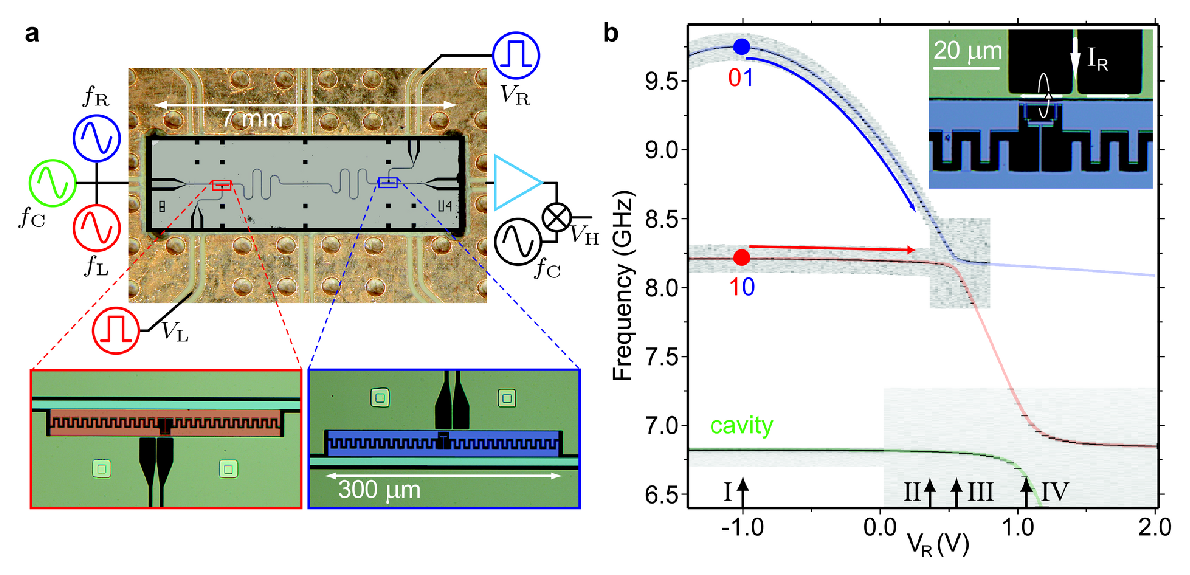
\includegraphics[height=0.8\textheight, trim={0 0 9.7cm 0}, clip]{Figure1_DeviceandSpec_LoRes}};
			\begin{scope}[x={(image.south east)},y={(image.north west)}]
				\node[MyBlue] at (0.7, 0.03) {\( T_1 = 1.3 \unit{\micro s} \)};
				\node[MyBlue] at (0.7, -0.06) {\( T_2^* = 1.8 \unit{\micro s} \)};
				\node[MyRed] at (0.3, 0.03) {\( T_1 = 0.8 \unit{\micro s} \)};
				\node[MyRed] at (0.3, -0.06) {\( T_2^* = 1.2 \unit{\micro s} \)};
			\end{scope}
		\end{tikzpicture}
	\end{frame}
	
	\begin{frame}[t]{Qubit spectrum}
		\begin{columns}
			\begin{column}{.5\textwidth}
				\vspace{.5cm}
				\begin{tikzpicture}[every node/.style={font=\scriptsize, align=left}]
					\node[anchor=south west,inner sep=0] (image) at (0,0) {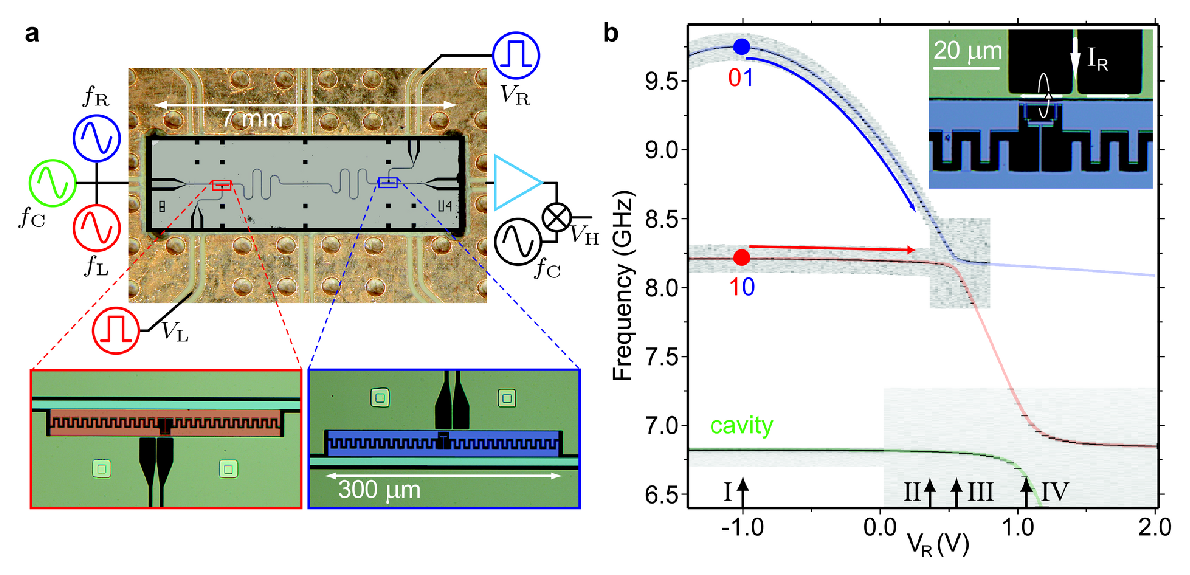
\includegraphics[height=0.7\textheight, trim={9.85cm 0 0 0}, clip]{Figure1_DeviceandSpec_LoRes}};
				\end{tikzpicture}
			\end{column}
			\uncover<2>{\begin{column}{.5\textwidth}
				\vspace{.3cm}\begin{figure}
					\hspace{.5cm}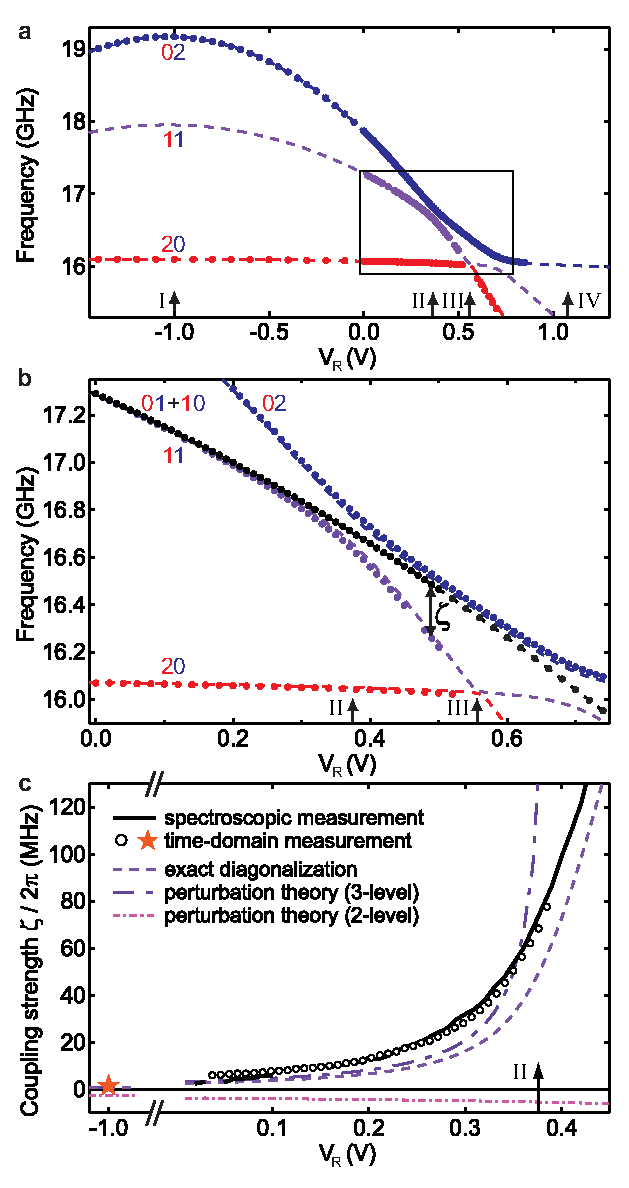
\includegraphics[height=0.675\textheight, trim={0 6.7cm 0 0}, clip]{Figure2_Zeta}
				\end{figure}
			\end{column}}
		\end{columns}
		
		
		
%		\begin{tikzpicture}
%			\node[anchor=south west,inner sep=0] (image) at (0,0) {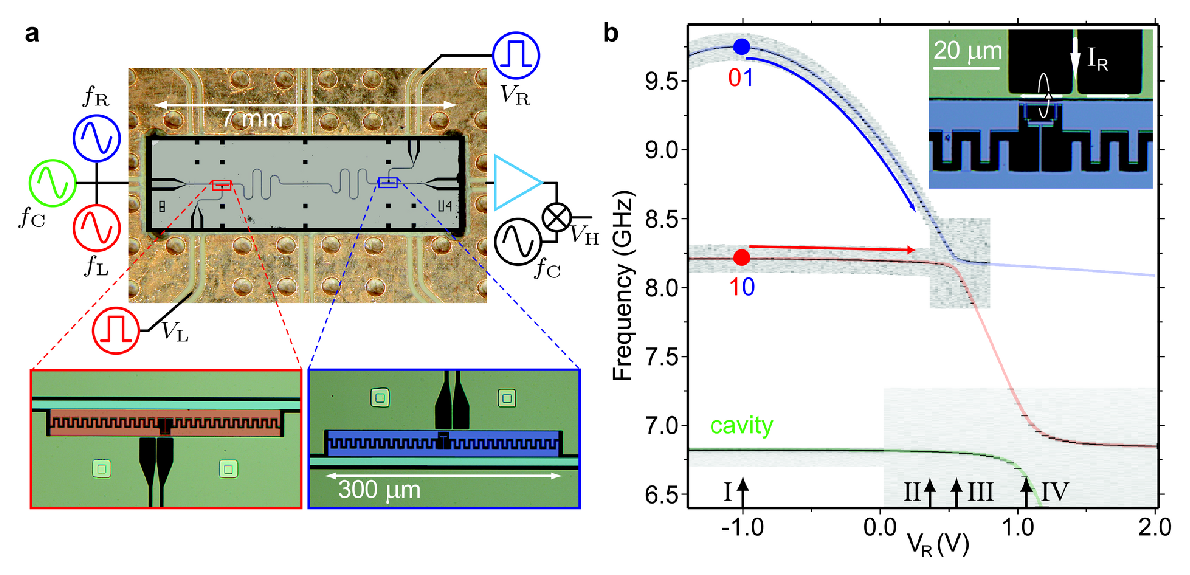
\includegraphics[height=0.8\textheight, trim={9.85cm 0 0 0}, clip]{Figure1_DeviceandSpec_LoRes}};
%			\node[anchor=south west,inner sep=0] (image) at (0,0) {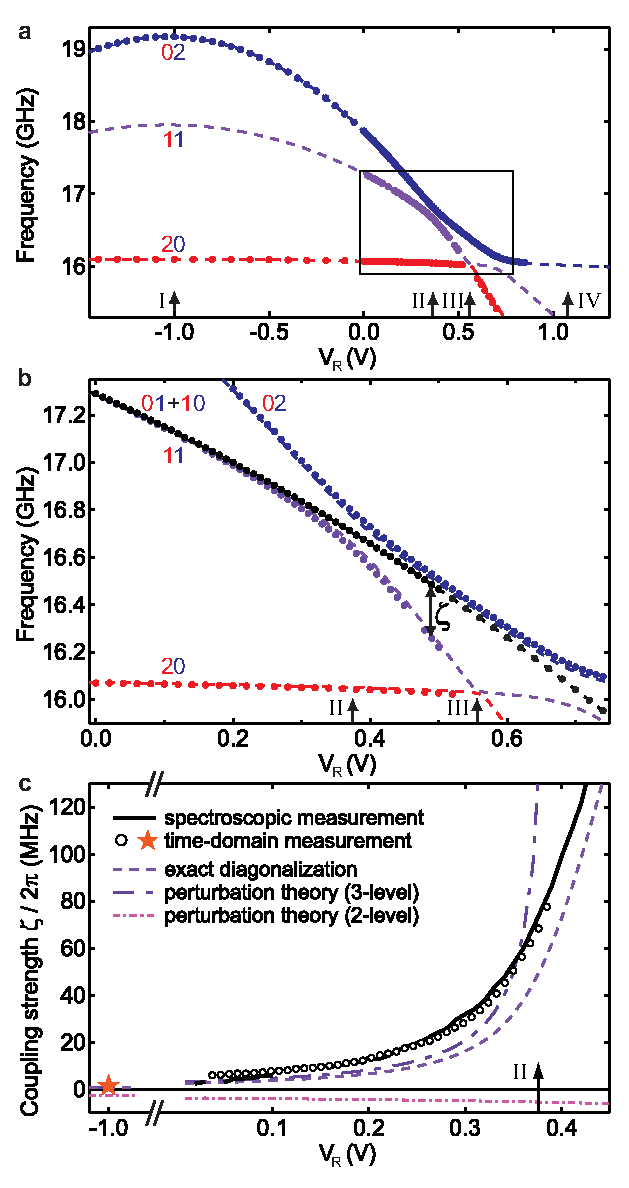
\includegraphics[height=0.8\textheight, trim={0 6.7cm 0 0}, clip]{Figure2_Zeta}};6
%			\begin{scope}[x={(image.south east)},y={(image.north west)}]
%%				\node[] at (0.335, -0.05) {\tiny\url{www.nobelprize.org}};
%			\end{scope}
%		\end{tikzpicture}
	\end{frame}
	

	\newcommand\MyBlue[1]{\color{MyBlue}#1}
	\newcommand\MyRed[1]{\color{MyRed}#1}
	
	\begin{frame}{CPhase gate}
%		\centering
		\begin{columns}
			\begin{column}{.5\textwidth}
				\begin{tikzpicture}
					\node[anchor=south west,inner sep=0] (image) at (0,0) {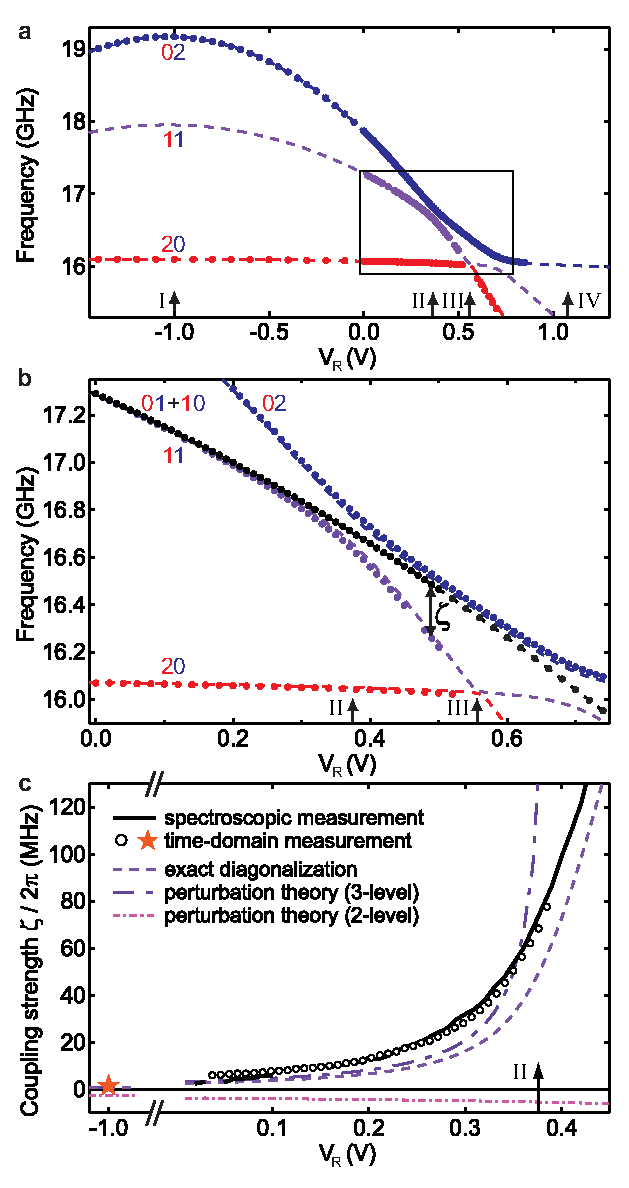
\includegraphics[height=0.8\textheight, trim={0 6.7cm 0 0}, clip]{Figure2_Zeta}};
%					\begin{scope}[x={(image.south east)},y={(image.north west)}]
%						
%					\end{scope}
				\end{tikzpicture}
			\end{column}
			\begin{column}{.5\textwidth}
				\begin{align*}
					\only<1>{U &= \begin{pmatrix}
							1 & 0 & 0 & 0\\
							0 & 1 & 0 & 0\\
							0 & 0 & 1 & 0\\
							0 & 0 & 0 & \expo[\iu \bm{\phi}_{\MyRed{1}\MyBlue{1}}]\\
					\end{pmatrix}}
					\only<2>{U &= \begin{pmatrix}
						1 & 0 & 0 & 0\\
						0 & \expo[\iu \bm{\phi}_{\MyRed{0}\MyBlue{1}}] & 0 & 0\\
						0 & 0 & \expo[\iu \bm{\phi}_{\MyRed{1}\MyBlue{0}}] & 0\\
						0 & 0 & 0 & \expo[\iu \bm{\phi}_{\MyRed{1}\MyBlue{1}}]\\
					\end{pmatrix}}\\[2em]
					\bm{\phi}_{\MyRed{l}\MyBlue{r}} &= 2\pi\uint{\delta f_{\MyRed{l}\MyBlue{r}}(t)}{t} \\
					\bm{\phi}_{\MyRed{1}\MyBlue{1}} &= \only<2>{\bm{\phi}_{\MyRed{0}\MyBlue{1}} + \bm{\phi}_{\MyRed{1}\MyBlue{0}}} - \uint{\zeta(t)}{t}
				\end{align*}
			\end{column}
		\end{columns}
	\end{frame}
	
	\begin{frame}{CPhase gate}
		\centering
		\begin{quotebox}
			\( cU_{ij} \ket{l,r} = (-1)^{\delta_{i\MyRed{l}} \delta_{j\MyBlue{r}}} \ket{l,r} \)
		\end{quotebox}\vspace{.5cm}
		\begin{columns}
			\begin{column}{.5\textwidth}
				\begin{tabular}{@{\extracolsep{5mm}} 
						l
						c
						c
						c
					}
					\toprule
					\makecell[t]{}
					&   {\makecell[t]{\( \bm{\phi}_{\MyRed{0}\MyBlue{1}} \)}}
					&   {\makecell[t]{\( \bm{\phi}_{\MyRed{1}\MyBlue{0}} \)}}
					&   {\makecell[t]{\( \bm{\phi}_{\MyRed{1}\MyBlue{1}} \)}}\\
					\midrule
					\( U_{00} \) & \( \pi \) & \( \pi \) & \( \pi \) \\
					\( U_{01} \) & \( \pi \) & \( 0 \) & \( 0 \) \\
					\( U_{10} \) & \( 0 \) & \( \pi \) & \( 0 \) \\
					\( U_{11} \) & \( 0 \) & \( 0 \) & \( \pi \) \\
					\bottomrule
				\end{tabular}
			\end{column}
			\begin{column}{.5\textwidth}
				\begin{align*}
					U &= \begin{pmatrix}
							1 & 0 & 0 & 0\\
							0 & \expo[\iu \bm{\phi}_{\MyRed{0}\MyBlue{1}}] & 0 & 0\\
							0 & 0 & \expo[\iu \bm{\phi}_{\MyRed{1}\MyBlue{0}}] & 0\\
							0 & 0 & 0 & \expo[\iu \bm{\phi}_{\MyRed{1}\MyBlue{1}}]\\
					\end{pmatrix}
				\end{align*}
			\end{column}
		\end{columns}
	\end{frame}
	
	\begin{frame}{Qubit entangling}
		\centering
		\hspace{-1cm}
		\begin{tikzpicture}[every node/.style={font=\scriptsize, align=left}]
			\node[anchor=south west,inner sep=0] (image) at (1,0) {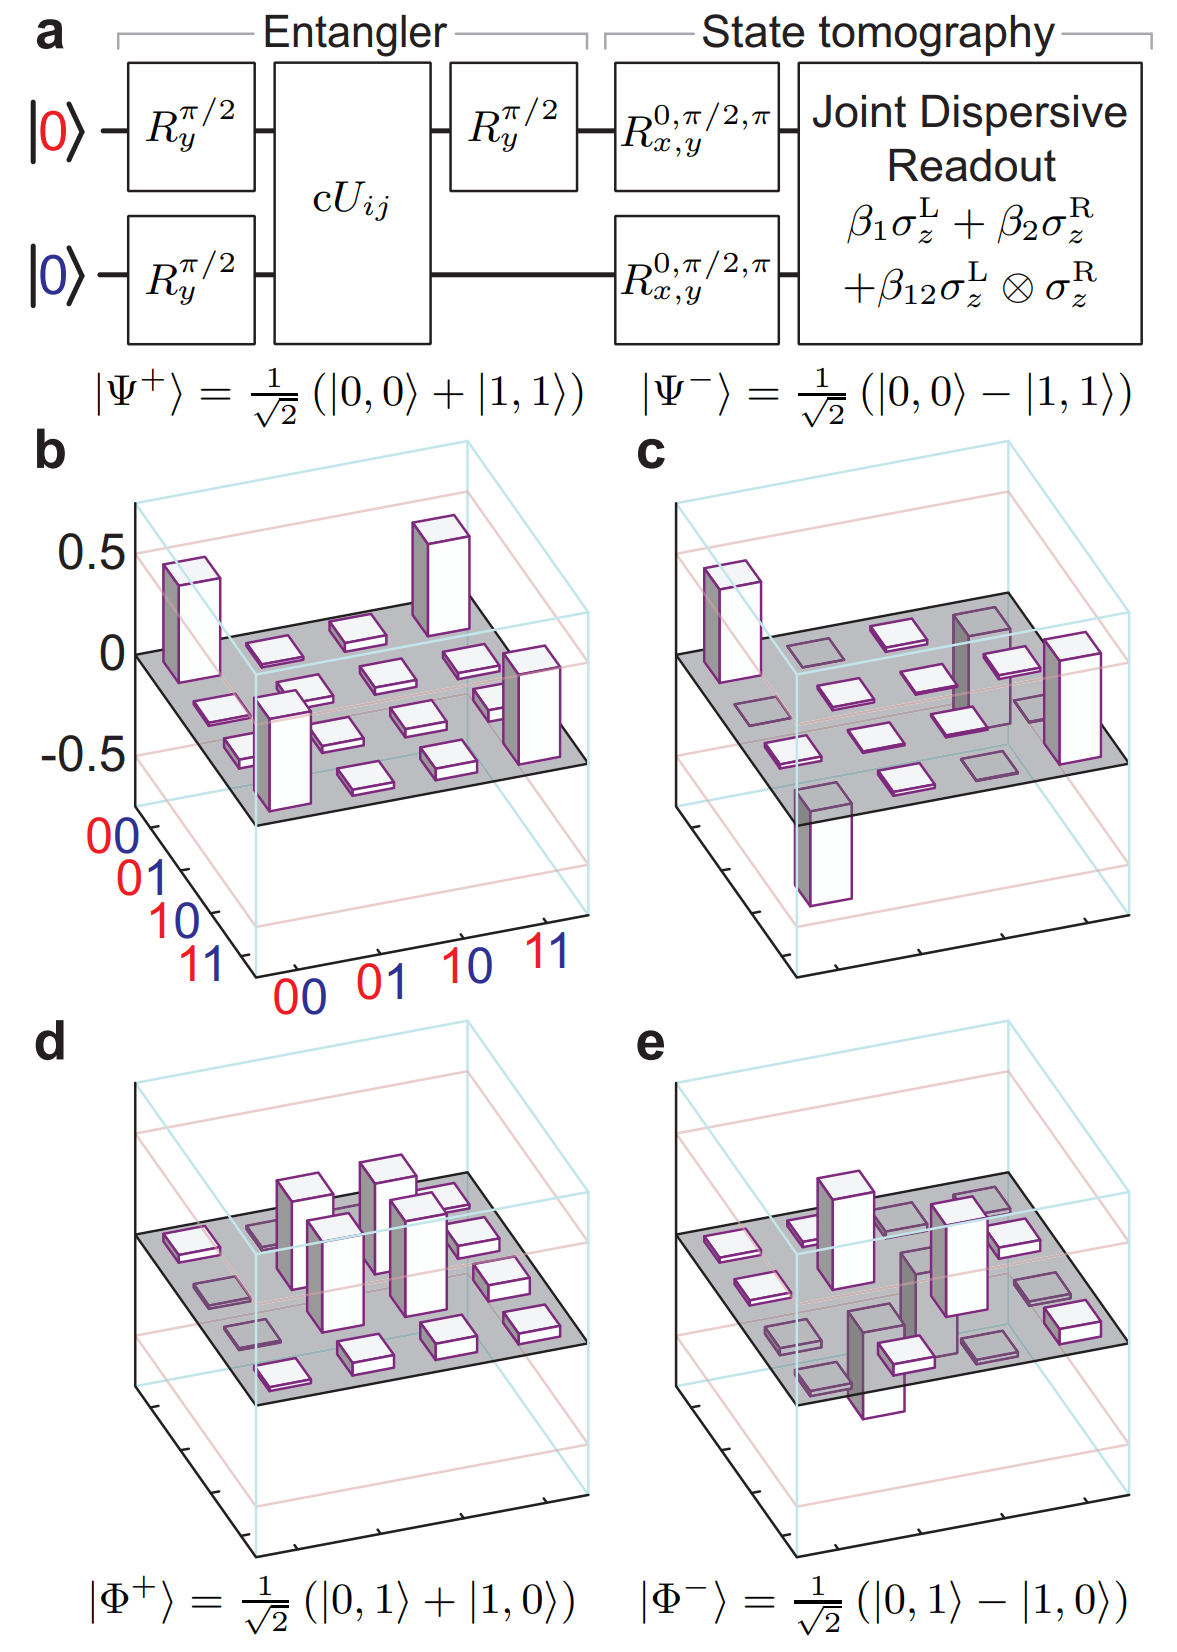
\includegraphics[height=.8\textheight, trim={0 0 0 0}, clip]{Bell}};
			
			\node at (7, 6) {\( N = 450 000 \)};
			
			\node at (7, 4) {\( F = 0.91(1) \)};
			\node at (7, 1) {\( F = 0.94(1) \)};
			\node at (0, 4) {\( F = 0.90(1) \)};
			\node at (0, 1) {\( F = 0.87(2) \)};
		\end{tikzpicture}
	\end{frame}
	
	\begin{frame}{Grover algorithm}
		\begin{figure}
			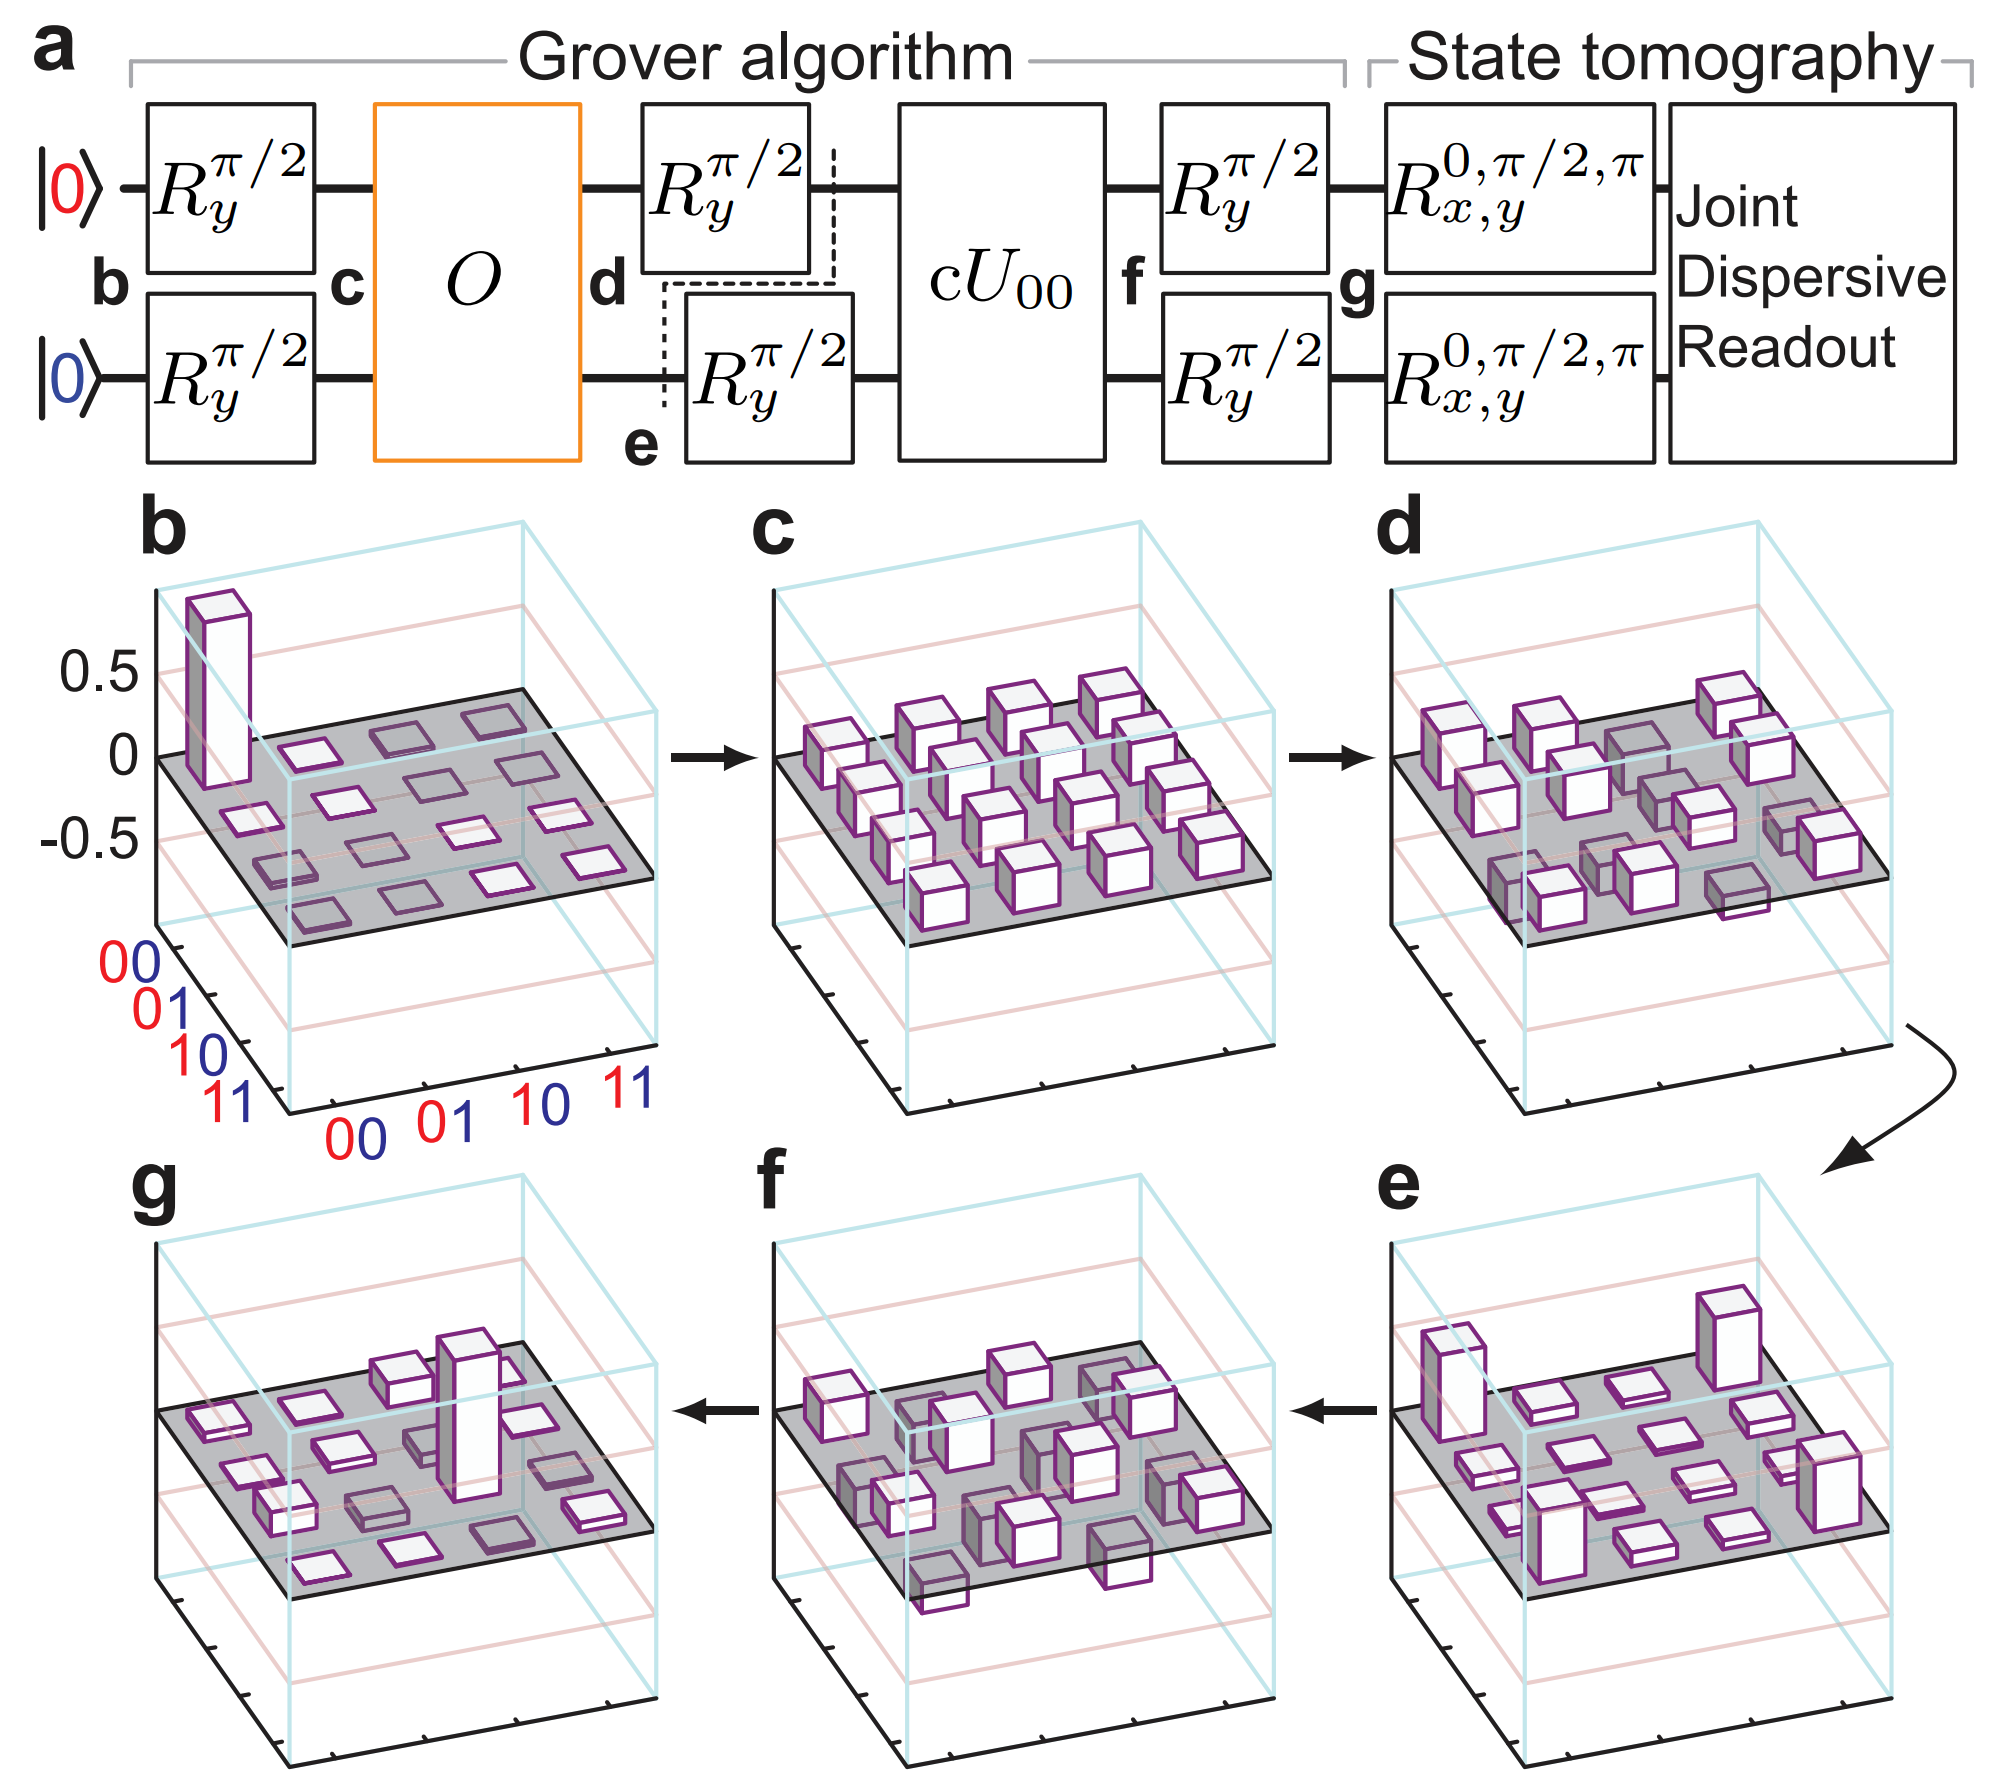
\includegraphics[height=.8\textheight, trim={0 0 0 0}, clip]{Grover}
		\end{figure}
	\end{frame}
	
	\begin{frame}{Results}
		\begin{figure}
			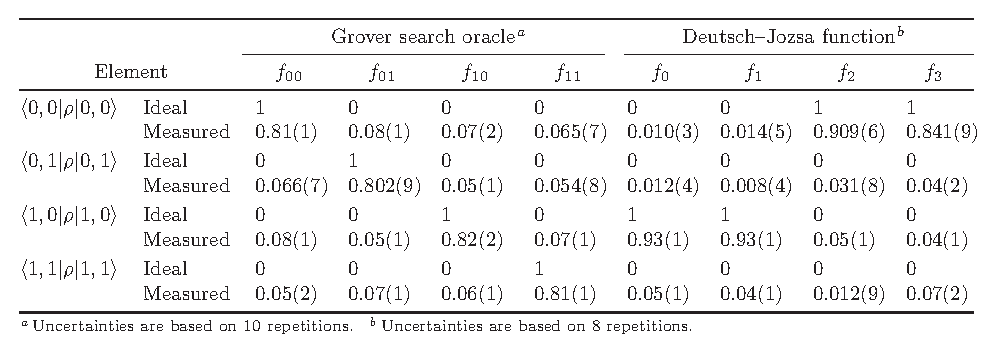
\includegraphics[width=\textwidth, trim={0 0 0 0}, clip]{Table}
		\end{figure}
	\end{frame}
	
	\begin{frame}{Outlook}
		\begin{tikzpicture}[scale=2.25, every node/.style={scale=0.8, black}, every path/.style={line width=1.15pt}]
			\draw[line width=1.5pt] (-0.15, 0) -- (4.15, 0);
			
			\draw[MyBlue, fill](0,0) circle (.045) node [below, yshift=-0.2cm] {\Large\( 1990 \)};
			\foreach \i in {0,...,3}{
				\draw[MyBlue, fill](1+\i,0) circle (.045) node [below, yshift=-0.2cm] {\Large\( 20\i0 \)};}
			
			\draw[MyBlue] (0.4, 0) -- (0.4, 0.35) node [left, xshift=0cm] {Shor (1994)};
			%			
%			\draw[MyBlue] (0.5, 0) -- (0.5, 0.5) node [above left, xshift=1cm] {Trapped ion CNOT (1995)};
			%			
			\draw[MyOrange] (0.9, 0) --++ (0, 0.85) node [above left, xshift=0.5cm] {First SC qubit (1999)};
			%			
%			\draw[MyBlue] (1.1, 0) --++ (0, 1.2) node [above left, xshift=0.5cm] {Rabi Oscillations (2001)};
			%			 
			\draw[MyBlue] (1.4, 0) --++ (0, 1.55) node [above left, xshift=0.5cm] {cQED (2004)};
			%			
			\draw[MyBlue] (1.7, 0) --++ (0, 1.9) node [above left, xshift=0.5cm] {Transmon (2007)};
			%			
			\draw[MyPurple] (1.9, 0) --++ (0, 2.4) node [above left, xshift=0.5cm] {2 qubit entanglement (2009)};
%			
			\draw[MyBlue] (2.1, 0) --++ (0, 2.4) node [above right, xshift=0cm] {DWave (2011)};
%			
			\draw[MyBlue] (2.3, 0) --++ (0, 2) node [above right, xshift=-0.5cm] {3D Transmon (2013)};
%			
			\draw[MyRed] (2.9, 0) --++ (0, 1.7) node [above, xshift=1.5cm] {\color{MyRed} Quantum supremacy \#1 (2019)};
%			
			\draw[MyBlue] (3.2, 0) --++ (0, 1.35) node [above right, xshift=-0.5cm] {127 Qubit (2022)};
%			
			\draw[MyBlue] (3.3, 0) --++ (0, 1) node [above right, xshift=-0.25cm] {433 Qubit (2023)};
%			
			\draw[MyBlue] (3.4, 0) --++ (0, 0.65) node [above right, xshift=-0.25cm] {1121 Qubit (2024)};
%			
			\draw[MyRed] (3.5, 0) --++ (0, 0.3) node [above right, yshift=-0.75cm, xshift=0cm, align=left] {\color{MyRed} Majorana Qubit*\\\color{MyRed} (2025)};
		\end{tikzpicture}	
	\end{frame}

	\begin{frame}[standout]
		\Huge Questions?
	\end{frame}
	
	\appendix
	
	\begin{frame}{Qubit readout}
		\begin{quotebox}
			\( H = \hbar\omega_r a^\dagger a + \frac{\hbar\omega_q}{2} \sigma_z + \hbar\chi a^\dagger a\sigma_z \quad\quad t(\omega_p) = \frac{\kappa}{\kappa + 2\iu (\omega_r^\mathrm{eff} - \omega_p)} \)
		\end{quotebox}
		
		\begin{columns}
			\begin{column}{.55\textwidth}
				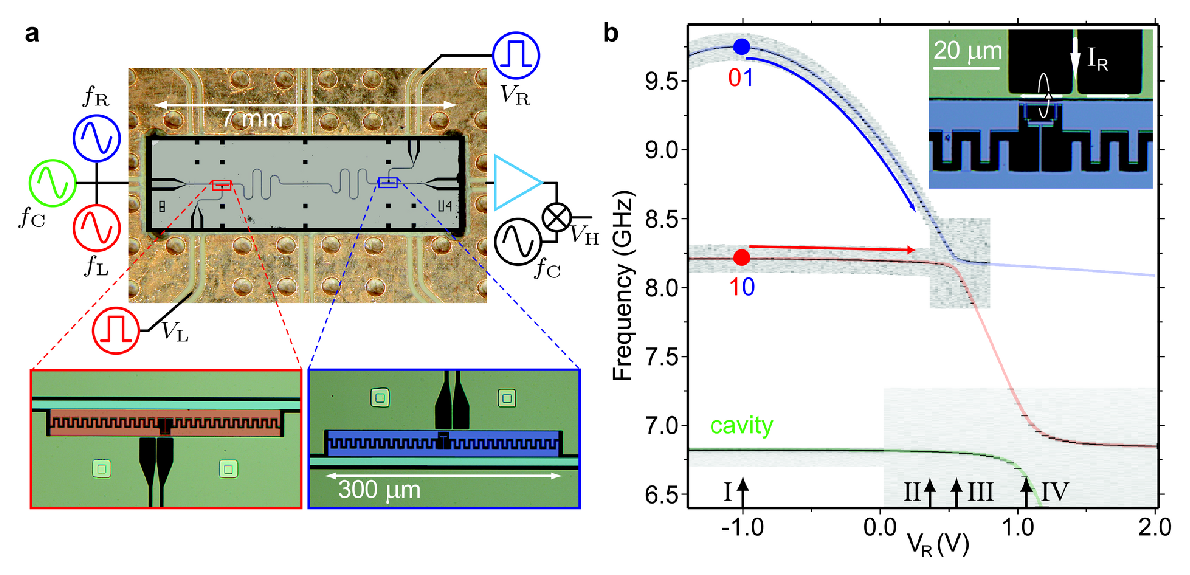
\includegraphics[height=0.6\textheight, trim={0 0 9.7cm 0}, clip]{Figure1_DeviceandSpec_LoRes}
			\end{column}
			\begin{column}{.4\textwidth}
				\begin{align*}
					s(t) &= A_s\cos(\omega t + \phi_s) \\
					\mathrm{LO}(t) &= A_\mathrm{LO}\cos(\omega t + \phi_\mathrm{LO}) \\
					V(t) &= s(t) \mathrm{LO}(t) \\
						&= A\cos(\phi_s - \phi_\mathrm{LO}) \\
						&+ \cos(2\omega t + \phi_s + \phi_\mathrm{LO})
				\end{align*}
			\end{column}	
		\end{columns}
	\end{frame}
	
	\begin{frame}{Pulses}
		\centering
		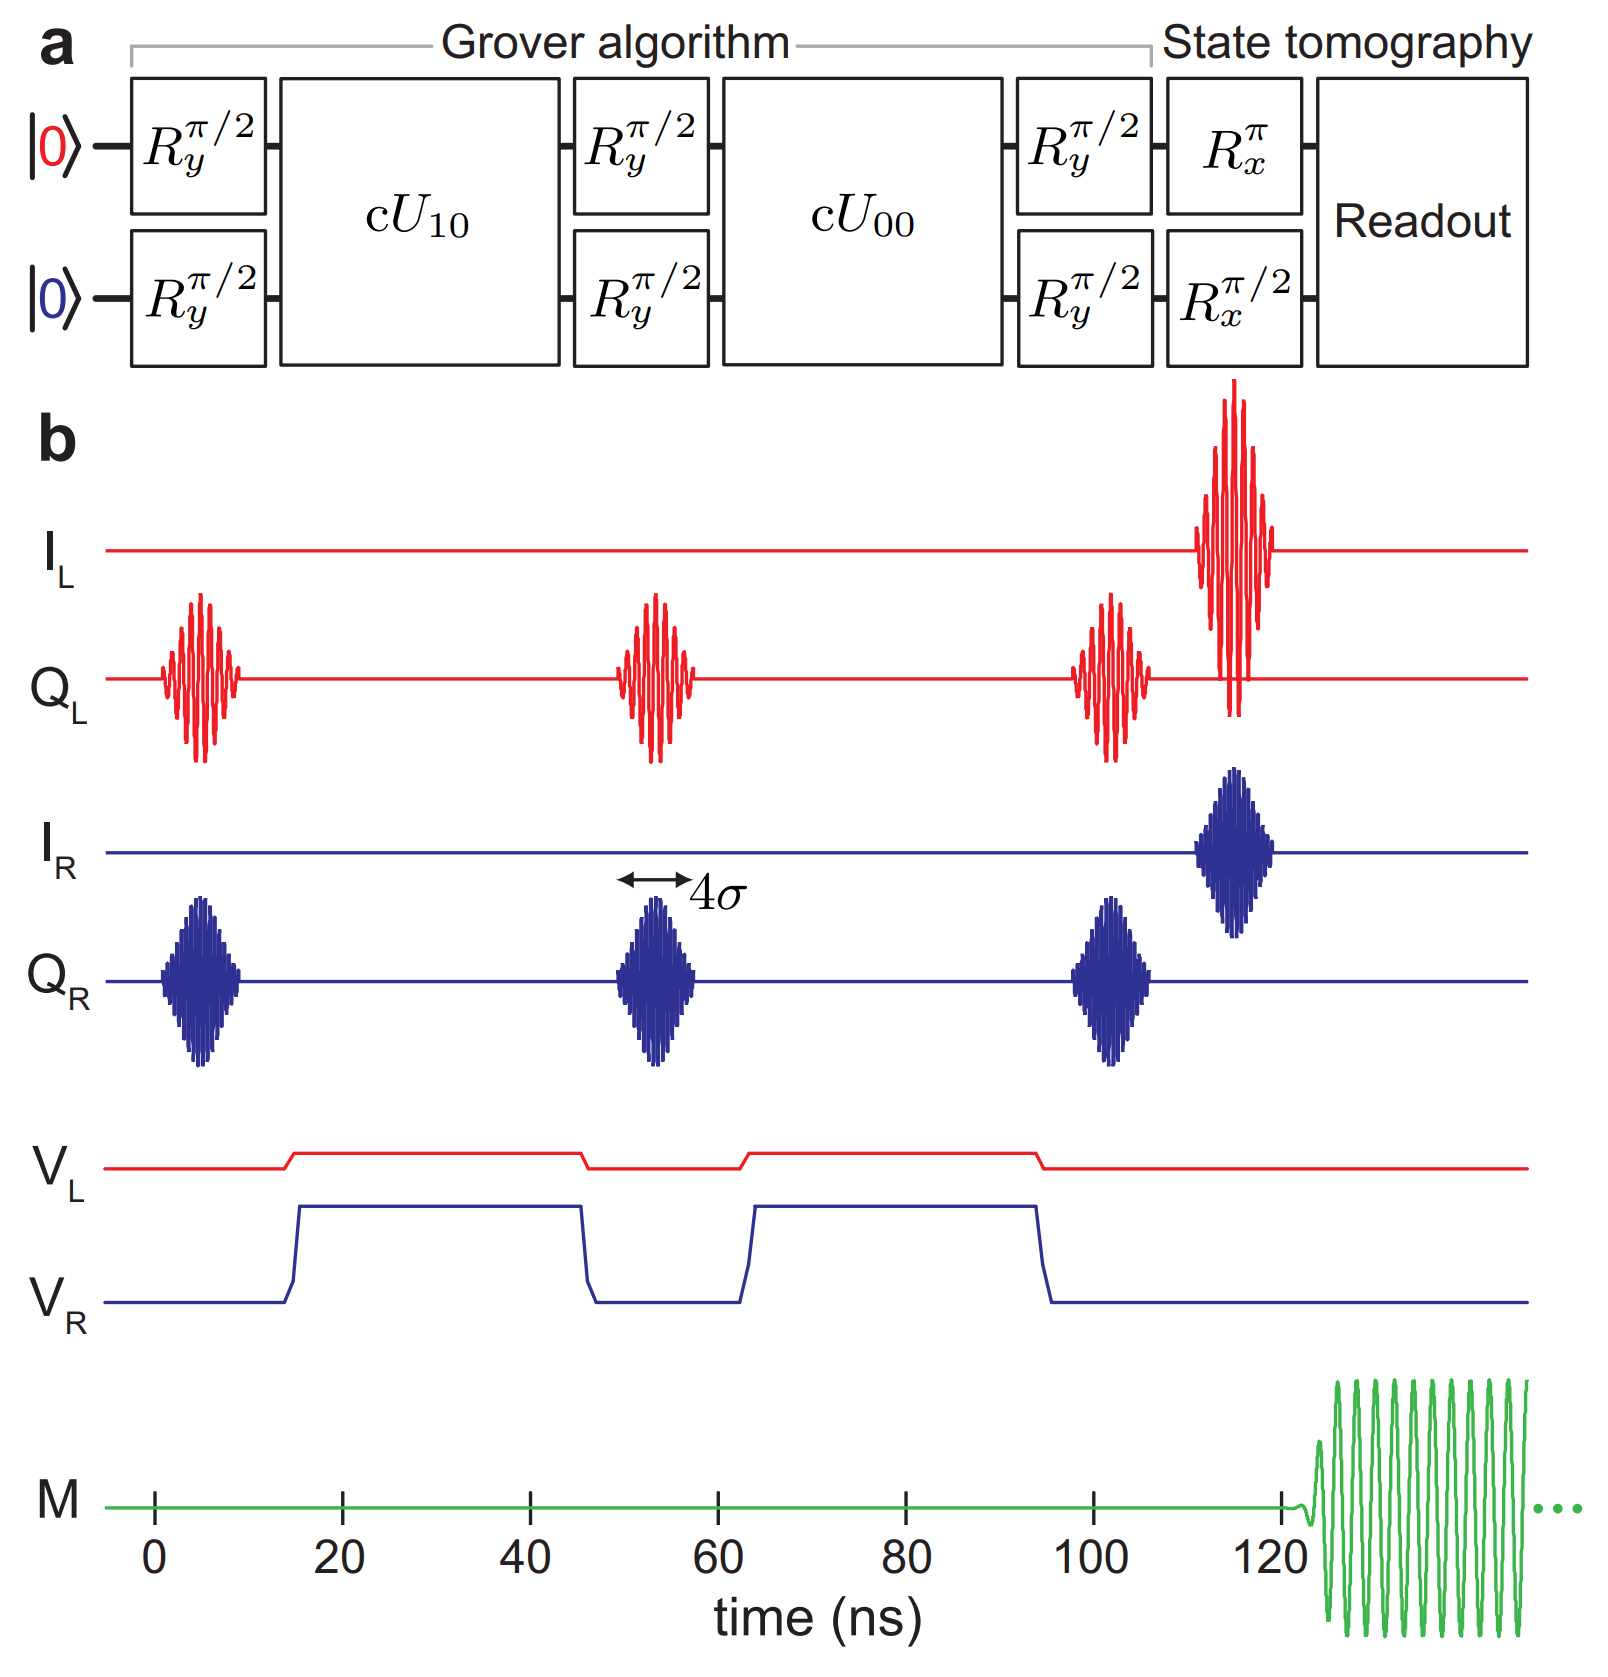
\includegraphics[height=.85\textheight]{Pulse}
	\end{frame}
	
	\begin{frame}{IQ modulation}
		\( M(t) = I(t)\cos(\omega t) + Q(t) \sin(\omega t) = A(t)\cos(\omega t + \phi(t)) \)
		\vspace*{.5cm}
		\begin{figure}
			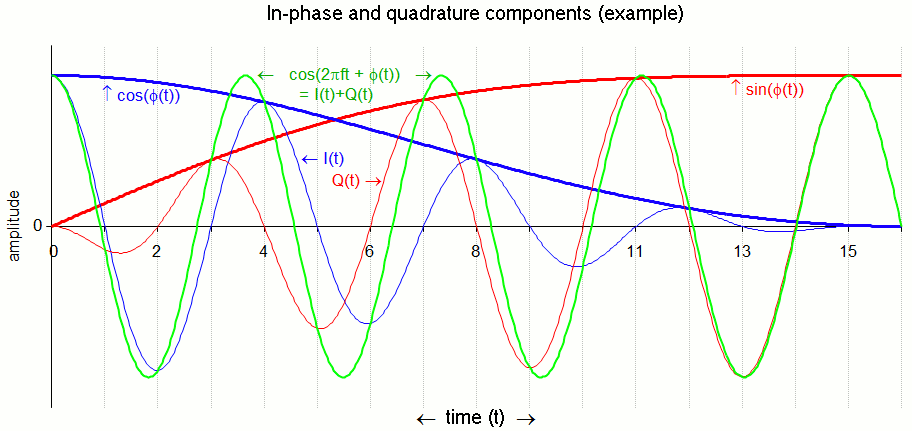
\includegraphics[width=\textwidth]{IQ}
		\end{figure}
	\end{frame}
	
	\begin{frame}[allowframebreaks]{Sources}
		\printbibliography
	\end{frame}
\end{document}